\section{BẤT PHƯƠNG TRÌNH BẬC NHẤT HAI ẨN}

\subsection{TÓM TẮT LÝ THUYẾT}
\subsubsection{Bất phương trình bậc nhất hai ẩn}
\begin{itemize}
	\item [\iconCH] Bất phương trình bậc nhất hai ẩn $x$, $y$ có dạng tổng quát là 
		\boxmini{$ax+by\le c \quad (1)$}
	trong đó $a$, $b$, $c$ là những số thực, $a$ và $b$ không đồng thời bằng $0$, $x$ và $y$ là các ẩn số.
	\item [\iconCH] Nghiệm của bất phương trình là những cặp số $(x_0;y_0)$ thỏa mãn (1).
	\item [\iconCH] Các dạng khác $ax+by<c$; $ax+by\ge c$; $ax+by>c$,...
\end{itemize}

\subsubsection{Biểu diễn tập nghiệm của bất phương trình bậc nhất hai ẩn}
\begin{itemize}
	\item [\iconCH] Các bất phương trình bậc nhất hai ẩn có vô số nghiệm. Để mô tả tập nghiệm của chúng, ta sử dụng phương pháp biểu diễn hình học.
	\item [\iconCH] Giả sử muốn biểu diễn miền nghiệm của bất phương trình $ax+by \le c \quad(2)$, ta thực hiện các bước như sau:
	\begin{boxdn}
		\begin{itemize}
			\item [\ding{172}] Trên mặt phẳng tọa độ $Oxy$, vẽ đường thẳng $\Delta \colon ax+by=c$.
			\item [\ding{173}] Lấy một điểm $M_0\left(x_0;y_0\right)$ không thuộc $\Delta$. Thay $(x_0;y_0)$ vào (2), sẽ có một trong hai trường hợp xảy ra: 
			\begin{itemize}
				\item Nếu mệnh đề đúng thì miền nghiệm phải chứa $M_0$. Suy ra nửa mặt phẳng bờ $\Delta$ (kể cả bờ $\Delta$) chứa $M_0$ là miền nghiệm của $(2)$.
				\item Nếu mệnh đề sai thì miền nghiệm không chứa $M_0$. Suy ra nửa mặt phẳng bờ $\Delta$ (kể cả bờ $\Delta$) không chứa $M_0$ là miền nghiệm của $(2)$.
			\end{itemize}
		\end{itemize}
	\end{boxdn}
\begin{note}
	Miền nghiệm của bất phương trình $ax+by<c$ là miền nghiệm của $ax+by \le c$ và bỏ đi đường thẳng $\Delta \colon ax+by=c$. Lúc này, khi vẽ đường thẳng $\Delta$, ta có thể dùng nét vẽ đứt để minh họa.
\end{note}
\end{itemize}
\begin{vidu}
	Biểu diễn hình học tập nghiệm của bất phương trình $2x+y\le 3 \quad(\star)$, ta làm như sau:\\
	\immini{
		\begin{itemize}
			\item [$\bullet$] Vẽ đường thẳng $\Delta\colon 2x+y=3$ qua hai điểm $(0;3)$ và $(1,5;0)$.
			\item [$\bullet$] Chọn $O\notin \Delta $. Thay tọa độ $O$ vào $(\star)$: $2 \cdot 0+0<3$ (thỏa).
			\item [$\bullet$]  Suy ra miền nghiệm của bất phương trình là nửa mặt phẳng bờ $\Delta$ chứa gốc tọa độ $O$ (miền không bị tô đậm trong hình vẽ).
		\end{itemize}
	}
	{
		\begin{tikzpicture}[line join=round, line cap=round, >=stealth,font=\footnotesize, scale=0.8]
			\fill [pattern=north east lines,pattern color=gray] (-0.5,4)--(3,4)--(3,-1) -- (2,-1)--cycle;
			\draw[samples=100,smooth,domain=-0.5:2,red] plot(\x,{-2*(\x)+3})node[left] {$\Delta$};
			\draw[->](-2,0)--(3.2,0) node[below] {$x$};
			\draw[->](0,-1)--(0,4.2) node[right] {$y$};
			\node (0,0) [below left]{$ O $};
			\foreach \x in {-1,...,2}
			\draw[shift={(\x,0)},color=black] (0pt,2pt) -- (0pt,-2pt);
			\foreach \y in {1,...,3}
			\draw[shift={(0,\y)},color=black] (2pt,0pt) -- (-2pt,0pt);
			\draw[fill=black] (0,3) circle(1pt) node[left]{$3$};
			\draw[fill=black] (1.5,0)circle(1pt) node[below left]{\tiny $\dfrac{3}{2}$};
		\end{tikzpicture}
	}
\end{vidu}
\subsection{RÈN LUYỆN KĨ NĂNG GIẢI TOÁN}

\begin{dang}{Biểu diễn miền nghiệm}	
\end{dang}
\begin{vd}
	Biểu diễn hình học tập nghiệm của bất phương trình bậc nhất hai ẩn sau:
	\begin{enumEX}[a)]{4}
		\item $3x + y \ge 3$.
		\item $2x - y \le 1$.
		\item $x + 2y > 33$.
		\item $2x - 4y < 8$.
	\end{enumEX}
	\loigiai{
		\textit{Quy ước: Miền nghiệm là phần mặt phẳng không bị gạch chéo.}
		
		\noindent
		\begin{minipage}{0.5\textwidth}
			\textbf{a) $3x + y \ge 3$}
			\begin{itemize}
				\item Vẽ $d_1: 3x + y = 3$.
				\item Thay $O(0;0) \Rightarrow 0 \ge 3$ (sai).
				\item Miền nghiệm \textbf{không chứa} $O$, \textbf{kể cả} bờ $d_1$.
			\end{itemize}
			\begin{center}
				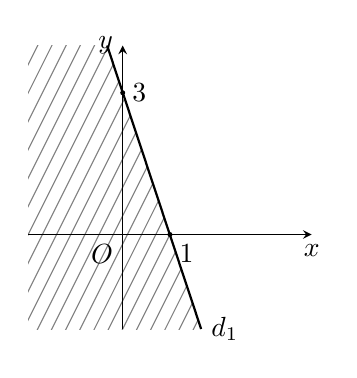
\begin{tikzpicture}[>=stealth, scale=0.6]
					\begin{scope}
						\clip (-2,-2) rectangle (4,4);
						% Phần bỏ đi là 3x+y < 3
						\clip (-2,9) -- (4,-9) -- (-4,-9) -- cycle;
						\foreach \i in {-10,-9.7,...,10} \draw[gray, thin] (\i,-10) -- (\i+10,10);
					\end{scope}
					\draw[->] (-2,0) -- (4,0) node[below] {$x$};
					\draw[->] (0,-2) -- (0,4) node[left] {$y$};
					\draw[thick] (-0.33, 4) -- (1.66, -2) node[right] {$d_1$};
					\node[below left] at (0,0) {$O$};
					\fill (1,0) circle (1.5pt) node[below right] {$1$};
					\fill (0,3) circle (1.5pt) node[right] {$3$};
				\end{tikzpicture}
			\end{center}
		\end{minipage}%
		\begin{minipage}{0.5\textwidth}
			\textbf{b) $2x - y \le 1$}
			\begin{itemize}
				\item Vẽ $d_2: 2x - y = 1$.
				\item Thay $O(0;0) \Rightarrow 0 \le 1$ (đúng).
				\item Miền nghiệm \textbf{chứa} $O$, \textbf{kể cả} bờ $d_2$.
			\end{itemize}
			\begin{center}
				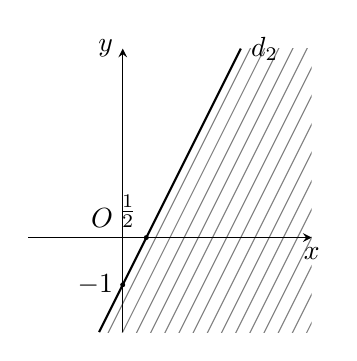
\begin{tikzpicture}[>=stealth, scale=0.6]
					\begin{scope}
						\clip (-2,-2) rectangle (4,4);
						% Phần bỏ đi là 2x-y > 1
						\clip (-2,-5) -- (4,7) -- (4,-5) -- cycle;
						\foreach \i in {-10,-9.7,...,10} \draw[gray, thin] (\i,-10) -- (\i+10,10);
					\end{scope}
					\draw[->] (-2,0) -- (4,0) node[below] {$x$};
					\draw[->] (0,-2) -- (0,4) node[left] {$y$};
					\draw[thick] (-0.5, -2) -- (2.5, 4) node[right] {$d_2$};
					\node[above left] at (0,0) {$O$};
					\fill (0,-1) circle (1.5pt) node[left] {$-1$};
					\fill (0.5,0) circle (1.5pt) node[above left] {$\frac{1}{2}$};
				\end{tikzpicture}
			\end{center}
		\end{minipage}
		
		\vspace{0.5cm}
		\noindent
		\begin{minipage}{0.5\textwidth}
			\textbf{c) $x + 2y > 33$}
			\begin{itemize}
				\item Vẽ $d_3: x + 2y = 33$ (nét đứt).
				\item Thay $O(0;0) \Rightarrow 0 > 33$ (sai).
				\item Miền nghiệm \textbf{không chứa} $O$, \textbf{không kể} bờ $d_3$.
			\end{itemize}
			\begin{center}
				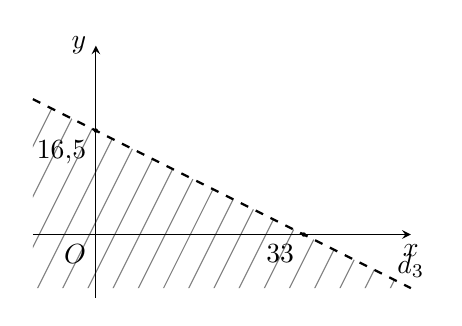
\begin{tikzpicture}[>=stealth, scale=0.08]
					\begin{scope}
						\clip (-10,-10) rectangle (50,30);
						% Phần bỏ đi là x+2y <= 33
						\clip (-10, 21.5) -- (50, -8.5) -- (-10, -8.5) -- cycle;
						\foreach \i in {-50,-46,...,50} \draw[gray, thin] (\i,-50) -- (\i+50,50);
					\end{scope}
					\draw[->] (-10,0) -- (50,0) node[below] {$x$};
					\draw[->] (0,-10) -- (0,30) node[left] {$y$};
					\draw[dashed, thick] (-10, 21.5) -- (50, -8.5) node[above] {$d_3$};
					\node[below left] at (0,0) {$O$};
					\fill (33,0) circle (10pt) node[below left] {$33$};
					\fill (0,16.5) circle (10pt) node[below left] {$16{,}5$};
				\end{tikzpicture}
			\end{center}
		\end{minipage}%
		\begin{minipage}{0.5\textwidth}
			\textbf{d) $2x - 4y < 8 \Leftrightarrow x - 2y < 4$}
			\begin{itemize}
				\item Vẽ $d_4: x - 2y = 4$ (nét đứt).
				\item Thay $O(0;0) \Rightarrow 0 < 4$ (đúng).
				\item Miền nghiệm \textbf{chứa} $O$, \textbf{không kể} bờ $d_4$.
			\end{itemize}
			\begin{center}
				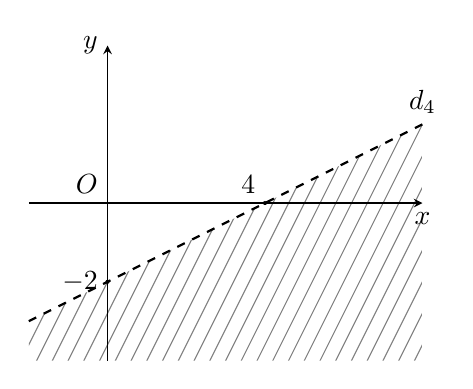
\begin{tikzpicture}[>=stealth, scale=0.5]
					\begin{scope}
						\clip (-2,-4) rectangle (8,4);
						% Phần bỏ đi là x-2y >= 4
						\clip (-2,-3) -- (8,2) -- (8,-4) -- (-2,-4) -- cycle;
						\foreach \i in {-10,-9.6,...,10} \draw[gray, thin] (\i,-10) -- (\i+10,10);
					\end{scope}
					\draw[->] (-2,0) -- (8,0) node[below] {$x$};
					\draw[->] (0,-4) -- (0,4) node[left] {$y$};
					\draw[dashed, thick] (-2, -3) -- (8, 2) node[above] {$d_4$};
					\node[above left] at (0,0) {$O$};
					\fill (4,0) circle (1.5pt) node[above left] {$4$};
					\fill (0,-2) circle (1.5pt) node[left] {$-2$};
				\end{tikzpicture}
			\end{center}
		\end{minipage}
	}
\end{vd}
\dongcham{24}

\begin{vd}
	Phần nửa mặt phẳng không bị gạch (không kể đường thẳng $d$) ở mỗi hình sau là miền nghiệm của bất phương trình nào?
	\begin{tasks}(2)
		\task \begin{tikzpicture}[line join=round, line cap=round, >=stealth,font=\footnotesize, scale=0.8]
			\fill[pattern=north east lines,pattern color=myblue] (-3,2.5)--(-3,-2)-- (4,-2)-- (4,-1)--cycle;
			\draw[samples=100,smooth,domain=4:-3,dashed] plot(\x,{-0.5*(\x)+1})node[above] {$d$};
			\draw[->](-3,0)--(4.5,0) node[below] {$x$};
			\draw[->](0,-2)--(0,3.3) node[right] {$y$};
			\node (0,0) [below right]{$ O $};
			\foreach \x in {-2,...,3}
			\draw[shift={(\x,0)},color=black] (0pt,2pt) -- (0pt,-2pt);
			\foreach \y in {-1,...,2}
			\draw[shift={(0,\y)},color=black] (2pt,0pt) -- (-2pt,0pt);
			\node[right] at (0,1.2) {$1$};
			\node[above] at (2,0) {$2$};
		\end{tikzpicture}
	\task \begin{tikzpicture}[line join=round, line cap=round, >=stealth,font=\footnotesize, scale=0.8]
		\fill [pattern=north west lines,pattern color=blue!60!green] (-1,-2)--(-3,-2)-- (-3,3)-- (1.5,3)--cycle;
		\draw[samples=100,smooth,domain=-1:1.5,dashed] plot(\x,{2*(\x)})node[right] {$d$};
		\draw[->](-3,0)--(3,0) node[below] {$x$};
		\draw[->](0,-2)--(0,3.3) node[right] {$y$};
		\node (0,0) [below right]{$O$};
		\foreach \x in {-2,...,2}
		\draw[shift={(\x,0)},color=black] (0pt,2pt) -- (0pt,-2pt);
		\foreach \y in {-1,...,2}
		\draw[shift={(0,\y)},color=black] (2pt,0pt) -- (-2pt,0pt);
		\draw[dashed](1,0)--(1,2)--(0,2);
		\draw[fill=black] (1,2)circle(1.5pt) node[right]{$M$};
	\end{tikzpicture}
	\end{tasks}
\loigiai{
\begin{enumerate}[a)]
	\item Đường giới hạn của miền nghiệm là trục tung có phương trình là $y=0$.\\
	Do miền nghiệm là phần bên phải trục tung nên ta có bất phương trình tương ứng là $y>0$.
	\item Gọi $d \colon y =ax+b$ là đường thẳng giới hạn. Theo hình vẽ thì $d$ qua hai điểm $(0;1)$ và $(2;0)$ nên ta có hệ
	$$\heva{&a \cdot 0 +b=1\\&a \cdot 2 +b=0} \Leftrightarrow \heva{&a=-\dfrac{1}{2}\\&b=1}.$$
	Vậy $d \colon y=-\dfrac{1}{2}x+1 \Leftrightarrow x+2y=2$.\\
	Do điểm $O(0;0)$ không thuộc miền nghiệm nên ta có bất phương trình tương ứng là $x+2y>2$.
	\item Gọi $d \colon y =ax+b$ là đường thẳng giới hạn. Theo hình vẽ thì $d$ qua hai điểm $(0;0)$ và $(1;2)$ nên ta có hệ
	$$\heva{&a \cdot 0 +b=0\\&a \cdot 1 +b=2} \Leftrightarrow \heva{&a=2\\&b=0}.$$
	Vậy $d \colon y=2x \Leftrightarrow 2x-y=0$.\\
	Do điểm $A(2;0)$ thuộc miền nghiệm nên ta có bất phương trình tương ứng là $2x-y>0$.
\end{enumerate}}
\end{vd} \dongcham{15}
\begin{dang}{Các bài toán thực tiễn}
\end{dang}
\begin{vd}
	Một gian hàng trưng bày bàn và ghế rộng $60\,m^2.$ Diện tích để kê một chiếc ghế là $0,5\,m^2$ , một chiếc bàn là $1,2\,m^2$ . Gọi $x$ là số chiếc ghế, $y$ là số chiếc bàn được kê.
	\begin{tasks}(1)
		\task Viết bất phương trình bậc nhất hai ẩn $x,\,y$ cho phần mặt sàn để kê bàn và ghế, biết diện tích mặt sàn dành cho lưu thông tối thiểu là $12\,m^2.$
		\task Chỉ ra ba nghiệm của bất phương trình trên.
	\end{tasks}
\loigiai{
	\begin{enumerate}[a)]
		\item Diện tích kê $x$ chiếc ghế là $0,5x$ m$^2$, ($x\in\mathbb{N^*}$).\\
		Diện tích kê $y$ chiếc ghế là $1,2y$ m$^2$, ($y\in\mathbb{N^*}$).\\
		Diện tích mặt sàn tối đa có thể kê bàn, ghế là $60-12=48$ m$^2$.\\
		Do đó ta có bất phương trình $0,5x+1,2y\le 48$.
		\item Cho $x=10$, ta được $1,2y \le 43$. Có thể chọn 3 giá trị $y_1=10$, $y_2=11$, $y_3=12$ thỏa mãn. Ba nghiệm của bất phương trình trên là $(10;10)$, $(10;11)$, $(10;12)$
	\end{enumerate}
	}
\end{vd} \dongcham{7}

\begin{vd}
	Hà, Châu, Liên và Ngân cùng đi mua trà sữa. Cả bốn bạn có tất cả $185$ nghìn đồng. Bốn bạn mua $4$ cốc trà sữa với giá tiền $35$ nghìn đồng một cốc. Các bạn gọi thêm trân châu cho vào trà sữa. Một phần trân châu đen có giá $5$ nghìn đồng, một phần trân châu trắng có giá $10$ nghìn đồng. Gọi $x, y$ lần lượt là số phần trân châu đen, trân châu trắng mà bốn bạn định mua thêm.
	\begin{enumerate}
		\item[a)] Viết bất phương trình bậc nhất hai ẩn $x, y$ để thể hiện số tiền các bạn có đủ khả năng chi trả cho phần trân châu đen, trắng.
		\item[b)] Chỉ ra một nghiệm nguyên của bất phương trình đó.
	\end{enumerate}
	\loigiai{
		\begin{enumerate}
			\item[a)] Số tiền bốn bạn dùng để mua $4$ cốc trà sữa (chưa kèm trân châu) là:
			$$ 4 \cdot 35 = 140 \text{ (nghìn đồng)}. $$
			Số tiền còn lại tối đa để các bạn có thể mua thêm trân châu là:
			$$ 185 - 140 = 45 \text{ (nghìn đồng)}. $$
			Số tiền cần trả để mua $x$ phần trân châu đen là $5x$ (nghìn đồng). \\
			Số tiền cần trả để mua $y$ phần trân châu trắng là $10y$ (nghìn đồng). \\
			Tổng số tiền dùng để mua thêm trân châu là $5x + 10y$ (nghìn đồng). \\
			Vì tổng số tiền mua trân châu không được vượt quá số tiền còn lại, ta có bất phương trình:
			$$ 5x + 10y \le 45. $$
			Chia cả hai vế của bất phương trình cho $5$, ta được bất phương trình thu gọn:
			$$ x + 2y \le 9. $$
			\textit{(Lưu ý điều kiện thực tế: $x, y \in \mathbb{N}$)}
			
			\item[b)] Dựa vào điều kiện thực tế, $x$ và $y$ phải là các số tự nhiên. Ta cần chọn một cặp số nguyên không âm $(x; y)$ thỏa mãn $x + 2y \le 9$. \\
			Ví dụ, chọn $x = 2$ và $y = 3$. \\
			Thay vào bất phương trình ta có: $2 + 2 \cdot 3 = 8 \le 9$ (luôn đúng). \\
			Vậy cặp số $(2; 3)$ là một nghiệm nguyên của bất phương trình (điều này có nghĩa là nhóm bạn có thể mua thêm $2$ phần trân châu đen và $3$ phần trân châu trắng).
			
			\textit{(Học sinh có thể chỉ ra các nghiệm nguyên khác như $(0; 0), (1; 1), (3; 2), \dots$ miễn sao thỏa mãn điều kiện $x, y \in \mathbb{N}$ và $x + 2y \le 9$).}
		\end{enumerate}
	}
\end{vd}
\dongcham{7}
\begin{vd}
	Nhân ngày Quốc tế Thiếu Nhi 1-6, một rạp chiếu phim phục vụ các khán giả một bộ phim hoạt hình. Vé được bán ra có hai loại:
	\begin{itemize}
		\item [$\bullet$] Loại 1 (dành cho trẻ từ 6-13 tuổi): 50 000 đồng/vé.
		\item [$\bullet$] Loại 2 (dành cho người trên 13 tuổi): 100 000 đồng/vé.
	\end{itemize}
	Người ta tính toán rằng, để không phải bù lỗ thì số tiền vé thu được ở rạp chiếu phim này phải đạt tối thiểu 20 triệu đồng. Hỏi số lượng vé bán được trong những trường hợp nào thì rạp chiếu phim phải bù lỗ?
	\loigiai{
	\immini{Gọi $x$ là số lượng vé loại 1 bán được, $y$ là số lượng vé loại 2 bán được $(x,y \in \mathbb{N})$.
	\begin{itemize}
		\item [$\bullet$] Số tiền bán vé thu được là $50x+100y$ (nghìn đồng).
		\item [$\bullet$] Người ta sẽ phải bù lỗ trong trường hợp $50x+100y<20 000$ hay $x+2y<400 \quad (1)$.
	\end{itemize}
	Miền nghiệm của (1) là những điểm có tọa độ nguyên nằm trong tam giác $OAB$. Vậy, nếu bán được $x$ vé loại 1 và $y$ vé loại 2 mà điểm $(x;y)$ nằm trong tam giác $OAB$ thì rạp phim phải bù lỗ.}{
	\begin{tikzpicture}[line join=round, line cap=round, >=stealth,font=\footnotesize, scale=0.5]
		\draw [pattern=dots,pattern color=myblue] (-3,3.5)--(5,3.5)-- (5,-0.5)--cycle;
		\draw[samples=100,smooth,domain=5:-3,red] plot(\x,{-0.5*(\x)+2})node[above] {$d$};
		\draw [color=white] (-3,3.5)--(5,3.5)-- (5,-0.5);
		\draw[->](-3,0)--(5.2,0) node[right] {$x$};
		\draw[->](0,-1)--(0,3.7) node[right] {$y$};
		\node (0,0) [below left]{$ O $};
		\foreach \x in {-2,...,3}
		\draw[shift={(\x,0)},color=black] (0pt,2pt) -- (0pt,-2pt);
		\foreach \y in {1,...,2}
		\draw[shift={(0,\y)},color=black] (2pt,0pt) -- (-2pt,0pt);
		\node[left] at (0,1.8) {$200$};
		\node[below] at (3.8,0) {$400$};
		\node[right] at (0,2.2) {$A$};
		\node[above] at (4.1,0) {$B$};
	\end{tikzpicture}
	}	
}
\end{vd} \dongcham{8}

\boxmini{BÀI TẬP TỔNG HỢP TỰ LUYỆN}

\begin{baitap}
	Phần nửa mặt phẳng không bị gạch (không kể đường thẳng $d$) ở mỗi hình sau là miền nghiệm của bất phương trình nào?
	\begin{enumEX}[a)]{3}
		\item \begin{tikzpicture}[line join=round, line cap=round, >=stealth,font=\footnotesize, scale=0.5]
			\fill[pattern=north west lines,pattern color=tsblue] (-3,0)--(-3,-2)-- (3,-2)-- (3,0)--cycle;
			\draw[->](-3,0)--(3,0) node[below] {$x$};
			\draw[->](0,-2)--(0,3) node[right] {$y$};
			\node (0,0) [below right]{$ O $};
			\foreach \x in {-2,...,2}
			\draw[shift={(\x,0)},color=black] (0pt,2pt) -- (0pt,-2pt);
			\foreach \y in {-1,...,2}
			\draw[shift={(0,\y)},color=black] (2pt,0pt) -- (-2pt,0pt);
		\end{tikzpicture}
		\item \begin{tikzpicture}[line join=round, line cap=round, >=stealth,font=\footnotesize, scale=0.5]
			\fill [pattern=north east lines,pattern color=myblue] (-1,3)--(-3,3)-- (-3,-2)-- (4,-2)--cycle;
			\draw[samples=100,smooth,domain=4:-1,dashed] plot(\x,{-(\x)+2})node[above] {$d$};
			%\draw [color=white] (-1,3)--(-3,3)-- (-3,-2)-- (4,-2);
			\draw[->](-3,0)--(4.5,0) node[below] {$x$};
			\draw[->](0,-2)--(0,3.3) node[right] {$y$};
			\node (0,0) [below right]{$ O $};
			\foreach \x in {-2,...,3}
			\draw[shift={(\x,0)},color=black] (0pt,2pt) -- (0pt,-2pt);
			\foreach \y in {-1,...,2}
			\draw[shift={(0,\y)},color=black] (2pt,0pt) -- (-2pt,0pt);
			\node[right] at (0,2.2) {$2$};
			\node[above] at (2.1,0) {$2$};
		\end{tikzpicture}
		\item \begin{tikzpicture}[line join=round, line cap=round, >=stealth,font=\footnotesize, scale=0.5]
			\fill [pattern=north west lines,pattern color=blue!60!green] (-3,-1.5)--(-3,3)-- (3,3)-- (3,1.5)--cycle;
			\draw[samples=100,smooth,domain=-3:3,dashed] plot(\x,{0.5*(\x)})node[right] {$d$};
			\draw[->](-3,0)--(3,0) node[below] {$x$};
			\draw[->](0,-2)--(0,3.3) node[right] {$y$};
			\node (0,0) [below right]{$O$};
			\foreach \x in {-2,...,2}
			\draw[shift={(\x,0)},color=black] (0pt,2pt) -- (0pt,-2pt);
			\foreach \y in {-1,...,2}
			\draw[shift={(0,\y)},color=black] (2pt,0pt) -- (-2pt,0pt);
			\draw[dashed](2,0)--(2,1)--(0,1);
			\draw[fill=black] (2,1)circle(1.5pt) node[above]{$M$};
		\end{tikzpicture}
	\end{enumEX}
	\loigiai{
		\begin{enumerate}[a)]
			\item Đường giới hạn của miền nghiệm là trục hoành có phương trình là $x=0$.\\
			Do miền nghiệm là phần bên trên trục hoành nên ta có bất phương trình tương ứng là $x>0$.
			\item Gọi $d \colon y =ax+b$ là đường thẳng giới hạn. Theo hình vẽ thì $d$ qua hai điểm $(0;2)$ và $(2;0)$ nên ta có hệ
			$$\heva{&a \cdot 0 +b=2\\&a \cdot 2 +b=0} \Leftrightarrow \heva{&a=-1\\&b=2}.$$
			Vậy $d \colon y=-x+2 \Leftrightarrow x+y=2$.\\
			Do điểm $O(0;0)$ không thuộc miền nghiệm nên ta có bất phương trình tương ứng là $x+y>2$.
			\item Gọi $d \colon y =ax+b$ là đường thẳng giới hạn. Theo hình vẽ thì $d$ qua hai điểm $(0;0)$ và $(2;1)$ nên ta có hệ
			$$\heva{&a \cdot 0 +b=0\\&a \cdot 2 +b=1} \Leftrightarrow \heva{&a=\dfrac{1}{2}\\&b=0}.$$
			Vậy $d \colon y=\dfrac{1}{2}x \Leftrightarrow x-2y=0$.\\
			Do điểm $A(2;0)$ thuộc miền nghiệm nên ta có bất phương trình tương ứng là $x-2y>0$.
	\end{enumerate}}
\end{baitap} \cham{25}

\begin{baitap}%[0D4B4-1]
	Biểu diễn miền nghiệm của các bất phương trình sau:
	\begin{enumEX}[a)]{3}
		\item $x-2y-1>0$;
		\item $x+y-1 \le 0$;
		\item $3x - y \le 0$;
		\item $-x+y+2>0$;
		\item $y+2\ge 0$;
		\item $-x+2\le 0$.
	\end{enumEX}
	\loigiai{
		\begin{enumerate}[a)]
			\item $x-2y-1>0$.
			\immini{
				Vẽ đường thẳng $\Delta \colon x-2y-1=0$ đi qua hai điểm $A(1;0)$ và $B\left(0;-\dfrac{1}{2}\right)$.\\
				Xét gốc tọa độ $O(0;0)$.\\
				Ta thấy $O \notin \Delta$ và $0-2 \cdot 0 -1<0$.\\
				Do đó miền nghiệm của bất phương trình là nửa mặt phẳng không kể bờ $\Delta$, không chứa gốc tọa độ $O$ (miền không gạch chéo trên hình bên).
			}{\vspace{-0.5cm}
				\begin{tikzpicture}[scale=1, font=\footnotesize, line join=round, line cap=round, >=stealth]
					\draw[->] (-3.6,0)--(3.8,0) node [below]{$x$};
					\draw[->] (0,-2)--(0,1.8) node [left]{$y$};
					\node at (0,0) [above left=-3pt]{$O$};
					\clip (-3.6,-2) rectangle (3.8,1.8);
					\fill[pattern=north west lines,opacity=0.6] plot[domain=-3.6:3.8](\x,{1/2*(\x)-1/2})--(3.8,1.8)--(-3.6,1.8)--cycle;
					\draw plot[domain=-3.6:3.8](\x,{1/2*(\x)-1/2})node[shift={(-120:10pt)}]{$\Delta$};
					\draw[fill=black] (1,0)circle(1pt) +(-5:8pt)node{$A$};
					\draw[fill=black] (0,-1/2)circle(1pt) +(-35:8pt)node{$B$};
					\node at (1,0)[shift={(-90:8pt)}]{$1$};
					\node at (0,-1/2)[shift={(-125:13pt)}]{$-\tfrac{1}{2}$};
				\end{tikzpicture}
			}
			\item $x+y-1\le 0$. 
			\immini{
				Vẽ đường thẳng $\Delta \colon x+y-1=0$ đi qua hai điểm $A(1;0)$ và $B(0;1)$.\\
				Xét gốc tọa độ $O(0;0)$.\\
				Ta thấy $O \notin \Delta $ và $0+0-1<0$.\\
				Do đó miền nghiệm của bất phương trình là nửa mặt phẳng kể cả bờ $\Delta$, chứa gốc tọa độ $O$ (miền không gạch chéo trên hình bên).
			}{\vspace{-0.5cm}
				\begin{tikzpicture}[scale=1, font=\footnotesize, line join=round, line cap=round, >=stealth]
					\draw[->] (-3.6,0)--(3.8,0) node [below]{$x$};
					\draw[->] (0,-2)--(0,1.8) node [left]{$y$};
					\node at (0,0) [below left=-3pt]{$O$};
					\clip (-3.6,-2) rectangle (3.8,1.8);
					\fill[pattern=north east lines,opacity=0.6] plot[domain=-3.6:3.8](\x,{-(\x)+1})--(3.8,1.8)--cycle;
					\draw plot[domain=-3.6:3](\x,{-(\x)+1})node[shift={(153:15pt)}]{$\Delta$};
					\draw[fill=black] (1,0)circle(1pt) +(65:8pt)node{$A$};
					\draw[fill=black] (0,1)circle(1pt) +(15:8pt)node{$B$};
					\node at (1,0)[shift={(-90:8pt)}]{$1$};
					\node at (0,1)[shift={(185:8pt)}]{$1$};
				\end{tikzpicture}
			}
			\item $3x - y \le 0$.
			\immini{
				Vẽ đường thẳng $d: 3x - y = 0 $.\\
				Thay tọa độ điểm $M(0;2)$ vào vế trái phương trình đường thẳng $(d)$, ta được: $-2 < 0$.\\
				Vậy miền nghiệm của bất phương trình là nửa mặt phẳng không chứa điểm $M$, kể cả bờ $(d)$. (Trên hình là nửa mặt phẳng không bị gạch bỏ).
			}{
				\begin{tikzpicture}
					%---------------------- Vẽ hệ trục tọa độ
					\draw[->] (-2.25,0)--(2.25,0) node[below right] {$x$};
					\draw[->] (0,-1.25)--(0,3.25) node[right] {$y$};
					\node (0,0) [above right]{$ O $};
					%----------------------- Vẽ đoạn chắn trên trục
					\foreach \x in {-2,-1,1}
					\draw[shift={(\x,0)},color=black] (0pt,2pt) -- (0pt,-2pt);
					%\node at (3.8,0.5) {$4$};
					\foreach \y in {-1,1,2,3}
					\draw[shift={(0,\y)},color=black] (2pt,0pt) -- (-2pt,0pt);
					%\node at (-0.5,-1.8) {$-2$};
					
					%--------------------- Vẽ hàm
					\draw [thick, domain=-.33:1, samples=100] plot (\x, {3*\x});
					\node at (.5,2.5) {$(d)$};
					
					%---------------------- Điểm M
					\fill (0,2) circle (2pt) node[left]{$M(0;2)$};
					
					%----------------------Vẽ miền nghiệm
					\tkzDefPoints{-.33/-.99/A, 2/-1/B, 2/3/C, 1/3/D}
					\tkzDrawPolygon[ pattern=north east lines,opacity=.3](A,B,C,D)
				\end{tikzpicture}
			}
		\item Bất phương trình $-x+y+2>0$.
		\immini{
			Vẽ đường thẳng $d_1\colon -x+y+2=0$ đi qua hai điểm $A(2;0)$ và $B(0;-2)$.\\
			Xét gốc tọa độ $O(0;0)\notin d_1$, ta có $-0+0+2>0$.\\
			Do đó, miền nghiệm của bất phương trình là nửa mặt phẳng không kể bờ $d_1$, chứa gốc tọa độ $O$ (miền không gạch chéo trên hình).}
		{\vspace{-1cm}
			\begin{tikzpicture}[line join=round, line cap=round,>=stealth,font=\footnotesize,scale=.7]
				\begin{scope}
					\clip (-1,-3) rectangle (4,3);
					\fill[pattern=north west lines] (-2,-4)--(6,-4)--(6,4)--cycle;
					\draw (5,3)--(-1,-3) node [pos=0.7, above] {$d_1$};
				\end{scope}
				\draw[->] (-1,0)--(4,0) node[below]{$x$};
				\draw[->] (0,-3)--(0,2) node[left]{$y$};
				\draw (0,0) node[below left]{$O$};
				\foreach \x in {2}
				\draw[thin] (\x,1pt)--(\x,-1pt) node [above] {$\x$};
				\foreach \y in {-2}
				\draw[thin] (1pt,\y)--(-1pt,\y) node [left] {$\y$};
			\end{tikzpicture}	
		}	
		\item Bất phương trình $y+2 \ge 0$.
		\immini{
			Vẽ đường thẳng $d_2\colon y+2=0$ đi qua điểm $C(0;-2)$ và song song trục hoành.\\
			Xét gốc tọa độ $O(0;0)\notin d_2$, ta có $0+2>0$.\\
			Do đó, miền nghiệm của bất phương trình là nửa mặt phẳng kể cả bờ $d_2$, chứa gốc tọa độ $O$ (miền không gạch chéo trên hình).}
		{\vspace{-1cm}
			\begin{tikzpicture}[line join=round, line cap=round,>=stealth,font=\footnotesize,scale=.7]
				\begin{scope}
					\clip (-2,-4) rectangle (3,1);
					\fill[pattern=north east lines] (-2,-2)--(-2,-4)--(3,-4)--(3,-2)--cycle;
					\draw (-2,-2)--(3,-2) node [pos=0.75, above, sloped] {$d_2$};
				\end{scope}
				\draw[->] (-2,0)--(3,0) node[below]{$x$};
				\draw[->] (0,-4)--(0,1) node[left]{$y$};
				\draw (0,0) node[below left]{$O$};
				\foreach \y in {-2}
				\draw[thin] (1pt,\y)--(-1pt,\y) node [above left] {$\y$};
			\end{tikzpicture}	
		}	
		\item Bất phương trình $-x+2 \le 0$.
		\immini{
			Vẽ đường thẳng $d_3\colon -x+2=0$ đi qua điểm $D(2;0)$ và song song với trục tung.\\
			Xét gốc tọa độ $O(0;0)\notin d_3$, ta có $-0+2>0$.\\
			Do đó, miền nghiệm của bất phương trình là nửa mặt phẳng kể cả bờ $d_3$, không chứa gốc tọa độ $O$ (miền không gạch chéo trên hình).}
		{\vspace{-1cm}
			\begin{tikzpicture}[line join=round, line cap=round,>=stealth,font=\footnotesize,scale=.7]
				\begin{scope}
					\clip (-1,-2) rectangle (4,2);
					\fill[pattern=north east lines] (2,-2)--(2,2)--(-1,2)--(-2,-2)--cycle;
					\draw (2,-2)--(2,2) node [pos=0.75,right] {$d_3$};
				\end{scope}
				\draw[->] (-1,0)--(4,0) node[below]{$x$};
				\draw[->] (0,-2)--(0,2) node[left]{$y$};
				\draw (0,0) node[below left]{$O$};
				\foreach \x in {2}
				\draw[thin] (\x,1pt)--(\x,-1pt) node [below right] {$\x$};
			\end{tikzpicture}	
		}	
		\end{enumerate}
	}
\end{baitap} \cham{42}

\begin{baitap}%[0D4B4]
	Hà mang $95000$ đồng ra chợ mua hoa cúc và hoa hồng. Một bông hoa cúc có giá $4000$ đồng, một bông hoa hồng có giá $7000$ đồng. Viết bất phương trình bậc nhất hai ẩn cho số tiền mà Hà phải chi để mua $x$ bông hoa cúc và $y$ bông hoa hồng.  
	\loigiai{
		Ta có $x, y\in\mathbb{N}^*$.\\
		Giá của $x$ bông hoa cúc là $4000x$ đồng, giá của $y$ bông hoa hồng là $7000y$ đồng.\\
		Vì số tiền Hà mang đi là $95000$ đồng nên ta có bất phương trình 
		\[4000x+7000y\le 95000\Leftrightarrow 4x+7y\le 95.\] 
	}
\end{baitap} \cham{7}

\begin{baitap}%[0D4K4]
	Một rạp chiếu phim $2$D phục vụ khán giả một bộ phim mới với $2$ loại vé khác nhau. Vé loại $1$ (từ thứ $2$ đến thứ $5$) giá $80000$ đồng/vé, vé loại $2$ (từ thứ $6$ đến chủ nhật và ngày lễ) giá $100000$ đồng/vé. Để không phải bù lỗ thì số tiền vé thu được ở rạp chiếu phim này phải đạt tối thiểu $150$ triệu đồng. Hỏi số lượng vé bán được trong những trường hợp nào thì rạp chiếu phim phải bù lỗ?
	\loigiai{
		Gọi $x$, $y$ lần lượt là số vé loại $1$, loại $2$ bán được ($x, y\in\mathbb{N}$).\\
		Tổng số tiền bán vé là $80x+100y$ nghìn đồng.\\
		Rạp chiếu phim phải bù lỗ trong trường hợp số tiền bán vé nhỏ hơn $150$ triệu đồng, tức là 
		\[80x+100y<150000\Leftrightarrow 4x+5y<7500.\quad\quad (1)\]
		\immini{
			Miền nghiệm của bất phương trình (1) được xác định như sau\\
			+/ Vẽ đường thẳng $d\colon 4x+5y=7500$.\\
			+/ Chọn gốc tọa độ $O(0;0)$ và tính $4\cdot0+5\cdot0<7500$.\\
			Do đó miền nghiệm của bất phương trình (1) là nửa mặt phẳng bờ $d$, chứa gốc tọa độ $O$, không kể đường thẳng $d$.\\
			Gọi $A$, $B$ lần lượt là giao điểm của $d$ và $Ox$, $Oy$. Khi đó, nếu bán được $x$ vé loại $1$ và $y$ vé loại $2$ mà điểm $(x;y)$ nằm trong miền tam giác $OAB$ không kể cạnh $AB$ thì rạp chiếu phim sẽ phải bù lỗ.
		}
		{
			\begin{tikzpicture}[scale=.7,>=stealth]
				\draw[->] (0,0) -- (5.3,0)node[below]{$x$};
				\draw[->,color=black] (0,0) -- (0,5.3)node[left]{$y$};
				\node[below left] at (0,0){$O$};
				\node[left] at (0,3){$1500$};
				\node[above right] at (0,3){B};
				\node[below] at (4,0){$1875$};
				\node[above] at (4,0){A};
				\clip(0,0) rectangle (5.3,5.3);
				\fill[pattern=north east lines](4,0)-- (5.3,0) -- (5.3,5.3) -- (0,5.3)--(0,3)-- cycle;
				\draw[line width=1.2pt,smooth,samples=100,domain=0:4] plot(\x,{-0.75 *(\x) +3});
			\end{tikzpicture}
		}	
	}
\end{baitap} \cham{10}
\begin{baitap}
Một cửa hàng bán lẻ bán hai loại hạt cà phê. Loại thứ nhất giá 140 nghìn đồng/kg và loại thứ hai giá 180 nghìn đồng/kg. Cửa hàng trộn $x$ kg loại thứ nhất và $y$ kg loại thứ hai sao cho hạt cà phê đã trộn có giá không quá 170 nghìn đồng/kg.
\begin{tasks}
	\task Viết bất phương trình bậc nhất hai ẩn $x, y$ thoả mãn điều kiện đề bài.
	\task Biểu diễn miền nghiệm của bất phương trình tìm được ở câu a trên mặt phẳng toạ độ.
\end{tasks}
\loigiai{
\begin{enumerate}[a)]
	\item Theo đề bài, ta có:
	$$
	140 x+180 y \leq 170(x+y).
	$$
	Bằng cách chuyển vế ta được bất phương trình bậc nhất hai ẩn $30 x-10 y \geq 0$ hay $3 x-y \geq 0$.
	\item Biểu diễn miền nghiệm của bất phương trình bậc nhất hai ẩn $3 x-y \geq 0$.
	\begin{itemize}
		\item [$\bullet$] Bước 1. Vẽ đường thẳng $d: 3 x-y=0$ trên mặt phẳng toạ độ.
		\item [$\bullet$] Bước 2. Lấy điểm $M(1 ; 0)$ không thuộc $d$ và điểm $M$ thoả mãn $3 \cdot 1-0=3>0$.
		Do đó, miền nghiệm của bất phương trình là nửa mặt phẳng bờ $d$ chứa điểm $M(1 ; 0)$.
	\end{itemize}
\begin{center}
	\begin{tikzpicture}[line join=round, line cap=round, >=stealth,font=\footnotesize, scale=0.7]
		\fill [pattern=north west lines,pattern color=blue!60!green] (-0.7,-2.1)--(-3,-2.1)-- (-3,3)-- (1,3)--cycle;
		\draw[samples=100,smooth,domain=-0.7:1,red] plot(\x,{3*(\x)})node[right] {$d$};
		\draw[->](-3,0)--(3,0) node[below] {$x$};
		\draw[->](0,-2.1)--(0,3.3) node[right] {$y$};
		\node (0,0) [below right]{$O$};
		\foreach \x in {-2,...,2}
		\draw[shift={(\x,0)},color=black] (0pt,2pt) -- (0pt,-2pt);
		\foreach \y in {-1,...,2}
		\draw[shift={(0,\y)},color=black] (2pt,0pt) -- (-2pt,0pt);
		\draw[fill=black] (1,0)circle(1.5pt) node[below]{$M$} node[above]{$1$};
	\end{tikzpicture}
\end{center}
\end{enumerate}}
\end{baitap}
\cham{18}